%label:"fig:admissibleHeegaardDiagram"
%author:JeffHicks
%name:"admissible HeegaardDiagram"
%type:"figure"
%parent:"def:weaklyAdmissibleHeegaardDiagram"
%caption:"An admissible Heegaard diagram"


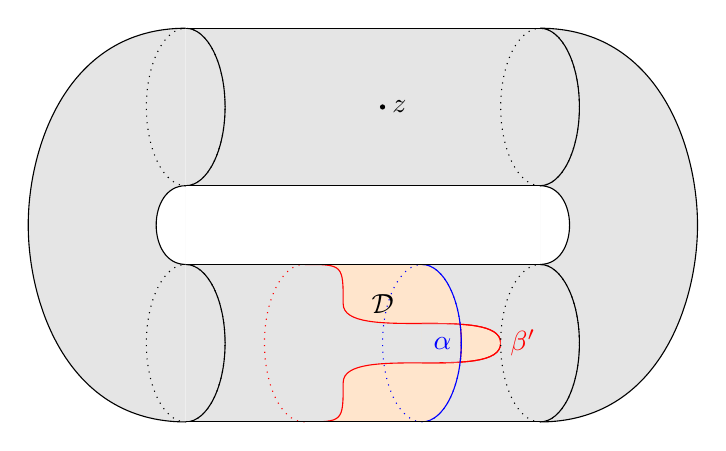
\begin{tikzpicture}

    \begin{scope}[]
    \begin{scope}[]
    
    \draw[fill=gray!20] (-2,-1.5) .. controls (-3.5,-1.5) and (-4,0) .. (-4,1) .. controls (-4,2) and (-3.5,3.5) .. (-2,3.5) (-2,1.5) .. controls (-2.5,1.5) and (-2.5,0.5) .. (-2,0.5);
    
    \end{scope}
    
    
    
    \begin{scope}[xscale=-1, shift={(-0.5,0)}]]
    
    \draw[fill=gray!20] (-2,-1.5) .. controls (-3.5,-1.5) and (-4,0) .. (-4,1) .. controls (-4,2) and (-3.5,3.5) .. (-2,3.5) (-2,1.5) .. controls (-2.5,1.5) and (-2.5,0.5) .. (-2,0.5);
    
    \end{scope}
    \fill[gray!20]  (-2,0.5) rectangle (2.5,-1.5);
    \fill[gray!20]  (-2,3.5) rectangle (2.5,1.5);
    
    \end{scope}
    
    \begin{scope}[]
    
    \fill[orange!20]  (1,-0.5) ellipse (0.5 and 1);
    \fill[orange!20]  (-0.5,0.5) rectangle (1,-1.5);
    \fill[gray!20]  (-0.5,-0.5) ellipse (0.5 and 1);
    \end{scope}
    
    
    \begin{scope}[]
    
    \draw[dotted]  (-2,-0.5) ellipse (0.5 and 1);
    \clip  (-2,0.5) rectangle (-1,-1.5);
    \draw  (-2,-0.5) ellipse (0.5 and 1);
    \end{scope}
    
    
    
    \begin{scope}[red, shift={(1.5,0)}]
    
    \draw[dotted]  (-2,-0.5) ellipse (0.5 and 1);
    \clip  (-2,0.5) rectangle (0.5,-1.5);
    \draw[fill=gray!20] (-2,0.5) .. controls (-1.5,0.5) and (-1.5,0.5) .. (-1.5,0) .. controls (-1.5,-0.5) and (0.5,0) .. (0.5,-0.5) .. controls (0.5,-1) and (-1.5,-0.5) .. (-1.5,-1) .. controls (-1.5,-1.5) and (-1.5,-1.5) .. (-2,-1.5);
    
    \clip  (-0.5,0) rectangle (0.5,-1);
    \draw[fill=orange!20] (-1.5,0) .. controls (-1.5,-0.5) and (0.5,0) .. (0.5,-0.5) .. controls (0.5,-1) and (-1.5,-0.5) .. (-1.5,-1);
    \clip (-1.5,0) .. controls (-1.5,-0.5) and (0.5,0) .. (0.5,-0.5) .. controls (0.5,-1) and (-1.5,-0.5) .. (-1.5,-1);
    
    \draw[fill=gray!20]  (-0.5,-0.5) ellipse (0.5 and 1);
    \draw (-1.5,0) .. controls (-1.5,-0.5) and (0.5,0) .. (0.5,-0.5) .. controls (0.5,-1) and (-1.5,-0.5) .. (-1.5,-1);
    
    \end{scope}
    
    
    \begin{scope}[blue, shift={(3,0)}]
    
    \draw[dotted]  (-2,-0.5) ellipse (0.5 and 1);
    \clip  (-2,0.5) rectangle (-0.5,-1.5);
    \draw  (-2,-0.5) ellipse (0.5 and 1);
    \end{scope}
    
    \begin{scope}[shift={(4.5,0)}]
    
    \draw[dotted]  (-2,-0.5) ellipse (0.5 and 1);
    \clip  (-2,0.5) rectangle (-1,-1.5);
    \draw  (-2,-0.5) ellipse (0.5 and 1);
    \end{scope}
    
    \begin{scope}[shift={(4.5,3)}]
    
    \draw[dotted]  (-2,-0.5) ellipse (0.5 and 1);
    \clip  (-2,0.5) rectangle (-1,-1.5);
    \draw  (-2,-0.5) ellipse (0.5 and 1);
    \end{scope}
    
    \begin{scope}[shift={(0,3)}]
    
    \draw[dotted]  (-2,-0.5) ellipse (0.5 and 1);
    \clip  (-2,0.5) rectangle (-1,-1.5);
    \draw  (-2,-0.5) ellipse (0.5 and 1);
    \end{scope}
    
    
    
    \node[right, red] at (2,-0.5) {$\beta'$};
    \node[left, blue] at (1.5,-0.5) {$\alpha$};
    \node at (0.5,0) {$\mathcal D$};
    
    \node[circle, fill=black, scale=.2] at (0.5,2.5) {};
    \node[right] at (0.5,2.5) {$z$};
    
    \draw (-2,-1.5) -- (2.5,-1.5) (-2,0.5) -- (2.5,0.5) (-2,1.5) -- (2.5,1.5) (-2,3.5) -- (2.5,3.5);
    
\end{tikzpicture}